\documentclass[12pt, a4paper]{article}
\usepackage[swedish]{babel}
\usepackage[T1]{fontenc}
\usepackage[utf8]{inputenc}
\usepackage{amsmath}
\usepackage{amssymb}
\usepackage{pgfplots}
\newcommand{\code}{\texttt}

\usepackage{graphicx}
\graphicspath{ {/home/mathias9807/c/Gymnasie-Projekt/Planer/graphics/} }

\linespread{1.3}
\pagenumbering{gobble}

\title{3D rymdspel}
\author{Mathias Johansson}


\begin{document}
	\maketitle
	
	\vfill
	
	\begin{center}
		{Gymnasiearbete 2016-2017 \hfill Peter Ågren \& David Nordqvist}
	\end{center}
	
	\begin{center}
		{De la Gardiegymnasiet, Lidköping \hfill Teknikprogrammet}
	\end{center}
	
	\newpage
	
	\begin{center}
		\Large\textbf{Abstract}
	\end{center}
	
	Modern games are often built using game engines, which let the developers focus more on building the games mechanics by abstracting away the hardware. However this hides the details in programming a game. To explore what goes into developing a complete game a simple 3D space game was built. The game would consist of flying a spaceship and trying to shoot down other AI controlled spaceships. It was constructed from the ground up using only the C programming language and various libraries. The result of the work was a working 3D game that looked mostly like the original game idea. The report showed that while certain games may benefit from the control of building a game from scratch, for most games a game engine let the developers focus more on building the game and less on fighting the platform. 
	
	\newpage
	
	\tableofcontents
	
	\newpage
	\pagenumbering{arabic}
	
	\section{Inledning}

	Moderna datorspel är väldigt komplicerade program. Att skapa ett spel involverar grafikprogrammering, simulation av fysik, inmatningshantering med mera. Det finns många spelmotorer och verktyg som förenklar hela skapandeprocessen men de gömmer även hur allting fungerar. Därför vill jag ta reda på vad som ingår i att programmera ett spel med 3D grafik från grunden utan hjälp av färdiga spelmotorer. 
	
	\subsection{Syfte och mål}
	
	Syftet med gymnasiearbetet är att ta reda på vad som ingår i att programmera ett tredimensionellt spel som innefattar alla funktioner som moderna spel har utan att ta hjälp av färdiga spelmotorer. Detta ska göras genom att ett spel programmeras från grunden. Spelet kommer vara ett tredimensionellt rymdspel där spelarens mål är att skjuta ner de andra skeppen. \\
	
	\noindent Gymnasiearbetet kopplas till följande examensmål:
	
	\begin{quote} \small
		Utbildningen ska utveckla elevernas kunskaper om och färdigheter i teknik och teknisk utveckling. Vidare ska utbildningen utveckla elevernas kunskaper om fysik och matematik med fokus på tekniska processer. I teknik ska eleverna undersöka, beskriva och systematisera olika egenskaper hos tekniska objekt och processer. Matematik är inom teknikområdet ett språk och ett redskap för att förstå, uttrycka och analysera sammanhang. 
	\end{quote}
	
	\subsection{Frågeställning}
	
	Frågeställningen som ska besvaras är: 

	\begin{center}
		Vilka svårigheter och problem finns i att programmera ett tredimensionellt spel från grunden utan hjälp av en spelmotor?
	\end{center}
	
	\subsection{Metod och material}
	
	För att organisera arbetet och för att få en bättre bild av hur arbetet fortskrider upprättas en tidsplan där en deadline sätts för varje stort delmål i projektet. För att organisera projektfilerna användes programmet \code{git}. Det är ett program som sparar all historik i ett projekt och säkerhetskopierar alla filer. 
	
	Under arbetets gång kommer hemsidor som stackoverflow.com och cpluslpus.com användas. Stackoverflow.com är en hemsida där användare kan lägga upp frågor om hur något fungerar och svara på andras frågor. Det finns ett stort arkiv av svarade frågor där alla de vanligaste sakerna folk undrar över har ett tydligt svar. Cplusplus.com är en hemsida som dokumenterar alla detaljer i C och C++ språken och förklarar hur de fungerar. I detta gymnasiearbete kommer en stor del bestå av att kontrollera datorns hårdvara, till exempel måste grafiken ritas genom grafikkortet, data måste läsas från disken och inmatningen måste läsas från tangentbordet. Detta görs genom programbibliotek, mindre program som är byggda för att underlätta skapandet av större program. OpenGL används för grafiken, SDL för inmatningen och OpenAL för ljud. För att få reda på hur varje bibliotek ska användas kommer respektive biblioteks dokumentation att användas. 
	
	\newpage
	\section{Genomförande}
	
	\subsection{Spelidé och verktyg}
	
	Arbetet började med att spelidéen utvecklades och att detaljerna fastställdes. Idéen med detaljerna skrevs ner i ett textdokument som senare användes som referens. Idéen var att skapa ett tredimensionellt rymdspel där spelaren styr ett rymdskepp. Målet i spelet är att skjuta ner de andra rymdskeppen. Om tiden finns ska även asteroider läggas till som skeppen också måste undvika. Det andra förberendande steget var att välja programmeringsspråk och verktyg. Som programmeringsspråk valdes C då det fungerar väl på flera olika plattformar. Ett viktigt programbibliotek som användes var \code{linmath.h}, ett litet bibliotek som förenklar vektor och matris hantering. Detta är användbart då det låter saker som positioner att lagras i en variabel (en vektor) istället för tre separata variabler (en X, Y och Z variabel). Vid det här steget bestämdes strukturen för hela spelmotorn. Då den består av så många olika delar (grafik, ljud, fysik, med mera) är det viktigt att koden är uppdelad i flera källkodsfiler. Det förenklar utvecklingen sent i arbetet. 
	
	\subsection{Hårdvarukommunikation}
	Det första av programmet som skrevs var det som direkt rörde datorns hårdvara, det vill säga grafik, tangentbordsinmatning och filinläsning med mera. Just grafiksystemet var den första delen som skrevs. Det första som programmet behövde göra var då att öppna ett fönster. Eftersom varje operativsystem öppnar fönster på ett eget sätt användes programbiblioteket \code{SDL} vilket hanterar skillnader mellan operativsystem åt programmeraren. När programmet kunde öppna ett fönster kunde den riktiga grafikkoden skrivas. Moderna datorer använder en separat grafikprocessor för att hantera 3D grafik och för att få bra prestanda behövde programmet kunna tala med grafikkortet. Detta görs med hjälp av en av flera tillgängliga API:er\footnote{Application Programming Interface, ett slags protokoll mellan program}. Den som användes heter OpenGL och valdes då den har störst support mellan operativsystem av alternativen. 
	
	\subsection{Inläsning av resurser}
	I spelet används texturer och modeller för att rita bakgrunden och rymdskeppen. De sparas i filer på hårddisken så för att programmet ska kunna använda dem måste grafiksystemet kunna läsa filerna. De filtyper som användes för texturer och modeller var PNG och COLLADA respektivt och för att läsa filerna användes programbiblioteken \code{assimp} och \code{stb\_image}. 
	
	\subsection{Inmatning}
	Näst skrevs tangentbordsinmatningen. Även den här delen behöver kommunicera mycket med operativsystemet men lyckligtvis hanterar \code{SDL} också inmatning. Internt ses tangentbordets knappar helt enkelt som en lista med sant/falskt värden där varje knapp på tangentbordet har ett eget värde. 
	
	\subsection{Fysik och rymdskepp}
	Vid det här stadiet fanns allt som behövdes för att lägga till skeppen och spelfysiken. Först skapades en datastruktur för skepp som innehåller en positionsvektor, en hastighetsvektor, en rotationsmatris plus en del andra variabler. Skeppets position beräknas enligt följande ekvation. 
	
	\begin{equation}
		p = p_0 + (\vec{r} * s) * \Delta t
	\end{equation}
	
	Där $p$ är den nya positionen på skeppet, $p_0$ är skeppets förra position och $s$ är skeppets fart. $\Delta t$ är tiden som har gått sedan förra gången positionen ändrades. Hastigheten fås genom att en vektor som pekar i riktningen som skeppet pekar i gångras med en fartskalär. 
	
	\subsection{Ljud}
	Efter att skeppen kunde styras skrevs ljudsystemet. SDL bibilioteket kan spela ljud men då det har väldigt få funktioner användes ett annat programbibliotek för ljud. OpenAL användes då det kan simulera många effekter som finns i verkligenheten, till exempel att ljud blir svagare över avstånd och dopplereffekten. I spelet spelas ett raketljud från varje rymdskepp. Som spelmekanik låter ljudet spelaren veta var de andra skeppen är och hur långt bort de är även när skeppen inte ligger inom spelarens vy. 
	
	\subsection{Partiklar}
	Nästa steg var att lägga till partiklar och skott. I spelet använder både avgaspartiklarna på rymdskeppen och skotten liknande datastrukturer vilket är anledningen till att de implementerades samtidigt. De båda har en textur, en position och en hastighet. Det speciella med partiklar är att när de renderas ska texturen alltid vara riktad mot kameran, då ser partikeln likadan ut från alla vinklar men det försvårar renderingen. Vid det här stadiet kan spelaren skjuta skott men då spelet inte hanterar kollisioner än kan skotten aldrig träffa något. Det skulle åtgärdas senare i arbetet. 
	
	\subsection{Menyer}
	Härnäst lades menyer till i spelet. För att rendera menyer behövde programmet först kunna rita ut texturer platt på skärmen och sedan rita text. Alla menyer ritas genom att en delvis genomskinlig texturerad polygon ställs framför kameran. Textrenderingen var mer komplicerad, för det användes ett ``font sheet''\footnote{En bild med varje bokstav i ASCII alfabetet utritat i ett rutnät i en given font}. När en bokstav skulle ritas beräknades först hur font texturen skulle förskjutas för att bokstaven skulle ligga längst upp och till vänster. Sedan klipptes texturen bort så att endast bokstaven var kvar vilken sedan ritades som vanligt. Detta upprepas för varje bokstav som skulle ritas. Med menysystemet klart visas nu en meny när spelet startas med spelets titel och några alternativ. Om spelet startas därifrån placeras spelaren och ett antal datorstyrda skepp i en cirkel också börjar matchen. 
	
	\subsection{Artificiell Intelligens}
	Det nästa steget till ett fungerande spel var att ge de andra skeppen AI\footnote{AI = Artificiell Intelligens}. Varje rymdskepp har i uppgift att skjuta ner så många andra skepp som möjligt så i deras AI-rutiner måste de först välja ett av skeppen som de ska sikta mot, sedan måste de svänga skeppet så att det pekar mot sitt mål och till sist om målet ligger ungefärligt rakt fram så ska de skjuta. Det första steget löstes genom att skeppen helt enkelt slumpade vilket av de andra skeppen som de tar som mål. Det andra steget löstes genom att skeppen kollar först om målet ligger över eller under det egna skeppet och i så fall svänger uppåt eller nerår respektivt, sedan gör samma i sidled. En viss marginal används där målet bedöms vara tillräckligt nära för att anses vara rakt framför skeppet. Om målet var innanför marginalerna så börjar skeppet skjuta. 
	
	\subsection{Kollisionshantering}
	En av de sista funktionerna som implementerades var kollisionsupptäckning. Detta krävs för att skotten ska kunna träffa något. Det finns många olika sätt att räkna ut om två föremål är i kontakt och mycket beror på vad föremålens former uppskattas som. Ett av de lättaste formerna att hantera är en så kallad ``Axis Aligned Bounding Box'' vilket är en kub som är låst till axlarna, det vill säga den kan inte rotera. Den form som valdes till det här spelet var en sfär eftersom den bättre uppskattar formerna som är inblandade och eftersom ekvationen som bestämmer om två sfärer kolliderar också är relativt simpel. 
	
	\begin{equation}
		d < r_A + r_B
	\end{equation}
	
	Alltså kolliderar sfärerna om avståndet $d$ mellan sfärernas mittpunkter är mindre än summan av sfärernas radier. $d$ räknas ut genom avståndsformeln:
	
	\begin{equation}
		d = \sqrt{(x_A - x_B)^2 + (y_A - y_B)^2 + (z_A - z_B)^2}
	\end{equation}
	
	I kodform såg algoritmen ut som följande när den användes för att jämföra punkten $b$ (ett skott) mot sfären $s$ (skeppet):
	
	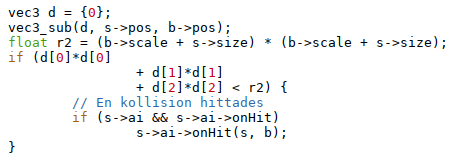
\includegraphics{collision-code.png}
	
	Först subtraheras föremålernas positioner vilket ger en vektor som går från ena föremålet till det andra. Sedan jämförs vektorns längd med sfärens radie. För att undvika att göra en kvadratrotsuträkning (vilket är en relativt långsam operation) jämförs de kvadrerade längderna istället för de riktiga längderna. 
	
	Varje spelcykel undersöks varje kobination av skott och skepp för att se om några kolliderar, i sådana fall sänks värdet på en räknare i skeppet som bestämmer skeppets HP. Vid det här stadiet var alla huvudsakliga funktioner färdiga och spelet mer eller mindre klart. 
	
	\newpage
	\section{Resultat}
	
	Spelet har nu alla av de viktiga funktionerna som spelet skulle ha när det var klart enligt den ursprungliga idén. Vissa funktioner fanns det inte tid för att implementera, till exempel asteroider. Samtidigt lades några nya idéer till som inte fanns i den originella designen så som en radar och sköldar på skeppen. Arbetet gick utan stora problem men även fast många programbibliotek användes som förenklade programmeringen var den delen som tog mest tid just grafik, ljud och inmatningen, det vill säga hårdvarusidan av programmet. En annan svår del var matematiken. Just att allting var i 3D gjorde arbetet betydligt mer komplicerat. Hårdvarukommunikationen och 3D matematiken är just det som en spelmotor sköter åt utvecklaren och därför skulle arbetet gått betydligt snabbare om en spelmotor använts. Slutsatsen med arbetet är att det svåra med att utveckla ett spel utan hjälp av en spelmotor är dels hårdvarokommunikationen och dels matematiken som går in i att göra spelet i 3D. 
	
	\newpage
	\section{Diskussion}
	
	Under arbetets gång behövde flera idéer tas bort på grund av tidsbrist. Som exempel var det först tänkt att det skulle finnas asteroider som skeppen behövde undvika. Att lägga till dem skulle dock involvera väldigt mycket kollisionskod för situationerna när två asteroider krockar och när skepp kraschar. Då asteroiderna skulle uppskattas som sfärer borde kollisionsupptäckarkoden kunna skrivas relativt snabbt. Dock skulle kollisionsresponsen vara mer komplicerad. Av samma anledning är skepp mot skepp kollisionen inte implementerad i den slutgiltiga versionen av spelet. 
	
	Slutsatsen var att eftersom en spelmotor sköter allt som berör datorns hårdvara skulle spelet blivit byggt mycket snabbare om en sådan hade använts. Allt det som tog längst tid i arbetet var sådant som en spelmotor skulle ge utvecklaren gratis. Utvecklaren skulle inte behöva oroa sig om att strukturera programmet på ett vettigt vis, detaljerna i att rendera delarna och all matematik som går in i att bygga spelet i 3D. Att bygga ett spel utan en färdig spelmotor kan dock låta spelutvecklaren att lättare lägga till vissa mer ovanliga funktioner men den stora majoriteten av spel kräver inget som en modern spelmotor inte klarar av. 
	
	\newpage
	\section{Referenslista}
	Hemsidor med dokumentation som har använts under arbetet: \\
	
	\noindent Khronos group. 2017. www.opengl.org. (Hämtad kontinuerligt från 06.2016 till 04.2017) \\
	Stack overflow. 2017. www.stackoverflow.com (Hämtad kontinuerligt från 06-2016 till 04.2017) \\
	CPlusPlus. 2017. www.cplusplus.com (Hämtad kontinuerligt från 06.2016 till 04.2017) \\
	Assimp. 2017. www.assimp.org (Hämtad kontinuerligt från 06.2016 till 08.2016) \\
	SDL. 2017. www.libsdl.org (Hämtad kontinuerligt från 06.2016 till 08.2016) \\
	
\end{document}
